
In this section, we look at some functions that are built-in to Matlab.  In a later section, we discuss how a user may write their own.

\section{Matlab: Built-In Functions}\label{sec:Matlab_builtin_functions}

As with most parts of Matlab, the Help window is useful in describing the functions that are in Matlab, Simulink, and any toolbox add-ons that you may have.  To access the entire list of functions, grouped in various ways, click on the Help button, the one shaped like a question mark at the top of the main Matlab window, or simply use the F1 button.  Once on the Help window, you can click on ``MATLAB Functions'' at the bottom.\\


\hspace{-.25in}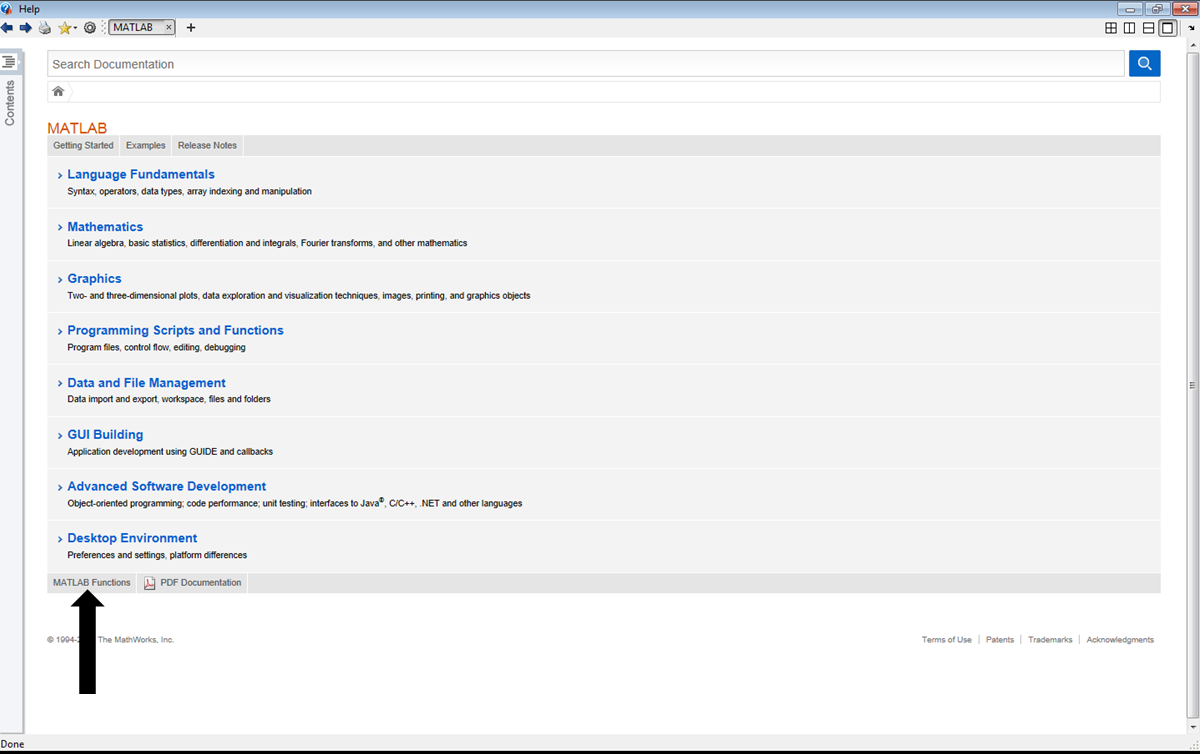
\includegraphics[scale=.6]{figures/matlab_function_reference2.png}

In discovering what a function does, we suggest to simply try it.  Let's start with the matrix \cour{A = [1 2 49 4;25 36 3 81]} and look at the output from several functions. First type in \\
\\
\noindent \cour{>> A = [1 2 49 4;25 36 3 81]}
\\
\\
\index{Matlab Functions!\cour{sqrt}}
$\bullet$ \cour{sqrt(A)} \\

The output:\\
\\
\cour{>> sqrt(A)}\\
\cour{ans =}\\
\cour{\ps 1.0000    1.4142    7.0000    2.0000}\\
\cour{\ps 5.0000    6.0000    1.7321    9.0000}\\
\\
is (hopefully) what you might expect.  It finds the square root of each of the entries.  If you know a little more linear algebra and was expecting the ``principal'' square root, or a matrix \cour{B} so that \cour{B * B = A}, this is created using \cour{B = sqrtm(A)}.\\
\\
\index{Matlab Functions!\cour{sin, sind}}
$\bullet$ \cour{sin(A), sind(A)}\\

The function \cour{sin(A)} finds the sine of every entry in \cour{A}, assuming the entries of \cour{A} are in radians:\\
\\
\cour{>> sin(A)}\\
\\
\cour{ans =}\\
\cour{\ps \po 0.8415    0.9093   -0.9538   -0.7568}\\
\cour{\ps -0.1324   -0.9918    0.1411   -0.6299}\\
\\
and the function \cour{sind(A)} does the same, but assumes the entries of \cour{A} are in degrees:\\
\\
\cour{>> sind(A)}\\
\\
\cour{ans =}\\
\cour{\ps 0.0175    0.0349    0.7547    0.0698}\\
\cour{\ps 0.4226    0.5878    0.0523    0.9877}\\

The other trigonometric functions are similarly named.\\
\\
\index{Matlab Functions!\cour{exp}}
\index{Matlab Functions!\cour{log,log10}}
$\bullet$ \cour{exp(A), log(A), log10(A)} \\

These three functions are base $e$ exponentiation, the natural log and the logarithm base 10.  They act entry-wise:\\
\\
\cour{>> exp(A)}\\
\\
\cour{ans =}\\
\cour{1.0e+035 *}\\
\cour{\ps 0.0000    0.0000    0.0000    0.0000}\\
\cour{\ps 0.0000    0.0000    0.0000    1.5061}\\
\\
\cour{>> log(A)}\\
\\
\cour{ans =}\\
\cour{\ps \phantom{00000}0    0.6931    3.8918    1.3863}\\
\cour{\ps 3.2189    3.5835    1.0986    4.3944}\\
\\
\cour{>> log10(A)}\\
\\
\cour{ans =}\\
\cour{\ps \phantom{00000}0    0.3010    1.6902    0.6021}\\
\cour{\ps 1.3979    1.5563    0.4771    1.9085}\\

We do see something curious here for the function \cour{exp(A)}.  It looks like all of the entries are zero until a closer look shows the 
leading term ``\cour{1.0e+035 *}''.  This means that every entry in the answer is multiplied by this factor $10^{35}$ (a rather large number).  The fact that the other entries look like zero is that there aren't enough decimal places to store each answer.\\
\\
\index{Matlab Functions!\cour{mean}}
\index{Matlab Functions!\cour{median}}
\index{Matlab Functions!\cour{std}}
$\bullet$ \cour{mean(A), median(A), std(A)}\\

These are some of the basic statistical functions.  The output for these are the mean, meadian, and standard deviation of the columns of \cour{A}.\\
\\
\cour{>> mean(A)}\\
\\
\cour{ans =}\\
\cour{\ps 13.0000   19.0000   26.0000   42.5000}\\
\\
\cour{>> std(A)}\\
\\
\cour{ans =}\\
\cour{\ps 16.9706   24.0416   32.5269   54.4472}\\
\\
\cour{>> median(A)}\\
\\
\cour{ans =}\\
\cour{\ps 13.0000   19.0000   26.0000   42.5000}\\
\\
\index{Matlab Functions!\cour{sort}}
\index{Matlab Functions!\cour{sortrows}}
$\bullet$ \cour{sort(A), sortrows(A)}\\

The command \cour{sort} rearranges the data in the columns of \cour{A} in increasing order.  The command \cour{sortrows} sorts the rows of \cour{A} in increasing order (determined by the first column).\\
\\
\cour{>> sort(A)}\\
\\
\cour{ans =}\\
\cour{\ps \po 1 \po 2 \po 3 \po 4}\\
\cour{\ps 25    36    49    81}\\
\\
\cour{>> sortrows(A)}\\
\\
\cour{ans =}\\
\cour{\ps \po 1 \po 2    49 \po4}\\
\cour{\ps 25    36     \po 3    81}\\

However, both of these functions can take other arguments.  For example, the \cour{sort} function can also be used to sort the columns, or can sort using either `descend' or `ascend'.  The \cour{sortrows} function can also be used to sort according to other columns.  See the Help files for more details.\\
\\    
\index{Matlab Functions!\cour{flipud}}
\index{Matlab Functions!\cour{fliplr}}
$\bullet$ \cour{flipud(A), fliplr(A)}\\

These two functions are abbreviations of ``flip up-and-down'' and ``flip left-to-right''.  That's exactly what they do:\\
\\
\cour{>> flipud(A)}\\
\\
\cour{ans =}\\
\cour{\ps 25    36  \po 3    81}\\
\cour{\ps \po 1 \po 2    49 \po4}\\
\\
\cour{>> fliplr(A)}\\
\\
\cour{ans =}\\
\cour{\ps \po 4    49 \po 2 \po 1}\\
\cour{\ps 81  \po 3    36    25}\\
\\    
\index{Matlab Functions!\cour{find}}
$\bullet$ \cour{find}\\

The function \cour{find} is used to located the position of values in a matrix.  \\ 
\\�
\cour{>> find(A==1)}\\
\\
\cour{ans =}\\
\cour{\ps 1}\\

A couple of comments about this example.  First, there is a double equals sign in \cour{A==1}.  There will be more about this in a future chapter (on relational operators), but you can read this as a question ``does \cour{A} equal 1?.'' The entire line \cour{find(A==1)} indicates the location where the (element of) \cour{A} does in fact equal 1 (namely the first entry).  Another example:\\
\\
\cour{>> find(a>5)}\\
\\
\cour{ans =}\\
\cour{\ps 2}\\
\cour{\ps 4}\\
\cour{\ps 5}\\
\cour{\ps 8}\\

Here we must again remember to read down the columns of \cour{A} to get to the 2nd, 4th, 5th and 8th entries.  We can tweak this last example to get the exact rows and columns containing entries greater than 5:\\
\\
\cour{>> [r,c]=find(A>5);[r,c]}\\
\\
\cour{ans =}\\
\cour{\ps 2     1}\\
\cour{\ps 2     2}\\
\cour{\ps 1     3}\\
\cour{\ps 2     4}\\

Here we have given the \cour{find} function two outputs to write to, the variables \cour{r} and \cour{c}, which are displayed together for easier reading using \cour{[r,c]}.  The output indicates that the entries of \cour{A} that are greater than $5$ can be found in the
2nd row \& 1st column, 2nd row \& 2nd column, 1st row \& 3rd column, and 2nd row \& 4th column.\\

\index{Matlab Functions!\cour{meshgrid}}
In the next example, we investigate the function \cour{meshgrid}.  The \cour{meshgrid} function is used to transform vectors \cour{x} and \cour{y} into arrays \cour{X} and \cour{Y} of sizes appropriate for computation and plotting.\\

\example{ex_meshgrid}{\textbf{Using \cour{meshgrid}}\\

Suppose we wanted to compute the area of a triangle for all possible combinations of the base, ranging from 7 to 10 units, and the height, ranging from 2 to 6 units.  Here's the set up (output suppressed):\\
\\
\cour{>> Base = 7:10;}\\ 
\cour{>> Height = 2:6;}\\

Now, we can't just multiply these two matrices together, nor can we ``dot multiply'' them either, since the dimensions of \cour{Base}, $1 \times 4$, and \cour{Height}, $1 \times 5$, do not line up properly in either case.  Instead we resize using \cour{meshgrid}:\\
\\
\cour{>> [NewBase,NewHeight] = meshgrid(Base,Height)}\\

This creates two matrices, \cour{NewBase} and \cour{NewHeight}, which are both $5 \times 4$.  We did not suppress the output, so one can see that these are:\\
\\
\\
\\
\cour{NewBase =}\\
\cour{\ps 7  8  9  10}\\
\cour{\ps 7  8  9  10}\\
\cour{\ps 7  8  9  10}\\
\cour{\ps 7  8  9  10}\\
\cour{\ps 7  8  9  10}\\
\\
and\\
\\
\cour{NewHeight =}\\
\cour{\ps 2 2 2 2}\\
\cour{\ps 3 3 3 3}\\
\cour{\ps 4 4 4 4}\\
\cour{\ps 5 5 5 5}\\
\cour{\ps 6 6 6 6}\\

We can now ``dot multiply'' them together:\\
\\
\cour{>> Area= (NewBase.*NewHeight)/2}\\
\\
\cour{Area =}\\
\\
\cour{\ps    \po7.0000   \po 8.0000   \po 9.0000   10.0000}\\
\cour{\ps    10.5000   12.0000   13.5000   15.0000}\\
\cour{\ps    14.0000   16.0000   18.0000   20.0000}\\
\cour{\ps    17.5000   20.0000   22.5000   25.0000}\\
\cour{\ps    21.0000   24.0000   27.0000   30.0000}\\
}\\

\newpage
\printexercises{exercises/03_exercises}

%EXERCISES:
%EXAMPLE:Generate  a matrix A containing 10,000 numbers from a Gaussian distribution with mean 80 and standard deviation 25. 
%
%Confirm that the mean is 80 by using the function \cour{mean}
%Confirm that the standard deviation is 25 by using the function \cour{std}
%Try the command \cour{hist(A,25)}


 
%\definition{def:lineintegral}{\textbf{TITLE}}
%
%\keyidea{idea:lineintprops}{\textbf{TITLE}}
%
%\printexercises{exercises/mathcad_introduction_exercises}
